\documentclass[12pt]{article}
\usepackage[utf8]{inputenc}
\usepackage{amsmath}
\usepackage{amssymb}
\usepackage{graphicx}
\usepackage{hyperref}
\usepackage{geometry}
\geometry{a4paper, margin=1in}
\usepackage{xcolor}
\usepackage{listings}
\usepackage{booktabs}

\title{\textbf{Deconstructing Spiking Neural Networks \\ Part 3: Same Accuracy. Half the Energy.}}
\author{Sovesh Mohapatra}
\date{\today}

\begin{document}

\maketitle

\section*{Introduction}
We have explored the continuous biology of the LIF neuron (Part 1) and built a full surrogate-gradient SNN in pure PyTorch (Part 2). The key question is: does a spiking network earn its biological complexity, and why should an ML practitioner care?

The answer is not in the accuracy column. It is in the energy column.

In this finale, we benchmark our custom \texttt{SNNClassifier} against a nearly parameter-identical ANN (MLP with ReLU) on MNIST over 10 epochs, and we compute the \textbf{effective inference energy cost} using Synaptic Operation (SOP) counting—the standard proxy used on neuromorphic hardware platforms.

\textbf{The headline result in advance}: At essentially the same accuracy ($\Delta = 0.47$ pp), the SNN achieves \textbf{51.7\% lower energy cost}—more than 2$\times$ more efficient at inference time.

\section*{The Benchmark Setup}

\subsection*{Task}
MNIST handwritten digit classification: 60,000 training images, 10,000 test images, 10 classes. Each $28 \times 28$ grayscale image is flattened to a 784-dimensional input vector, normalized with the MNIST mean and standard deviation (0.1307, 0.3081).

\subsection*{Model Architectures}
Both models share a hidden dimension of 256 neurons, a batch size of 256, and are trained with the Adam optimizer at a learning rate of $10^{-3}$ for 10 epochs.

\begin{table}[h]
\centering
\begin{tabular}{@{}lccc@{}}
\toprule
\textbf{Model} & \textbf{Architecture} & \textbf{Parameters} & \textbf{Timesteps $T$} \\
\midrule
ANN (MLP) & Linear(784,256)$\to$ReLU$\to$Linear(256,256)$\to$ReLU$\to$Linear(256,10) & 269,322 & --- \\
SNN (LIF) & Linear(784,256)$\to$LIF$\to$Linear(256,256)$\to$LIF$\to$Linear(256,10) & 269,834 & 25 \\
\bottomrule
\end{tabular}
\caption{Model architectures. Parameter counts differ by less than 0.2\%, ensuring a fair comparison. The SNN runs $T=25$ simulation timesteps per input sample.}
\end{table}

\section*{Accuracy Results}

\begin{table}[h]
\centering
\begin{tabular}{@{}lccc@{}}
\toprule
\textbf{Model} & \textbf{Params} & \textbf{Train Acc.} & \textbf{Test Acc.} \\
\midrule
ANN (MLP) & 269,322 & 99.52\% & 97.92\% \\
SNN (LIF) & 269,834 & 98.70\% & 97.45\% \\
\bottomrule
\end{tabular}
\caption{Final accuracy after 10 epochs on MNIST. The SNN matches the ANN within 0.47 percentage points. With more training epochs, threshold-balancing, or temporal ensembling, this gap closes further.}
\end{table}

The accuracy gap of 0.47 percentage points is not the story here. Both models are competitive classifiers. The question is: \textit{at what cost?}

\section*{The Energy Argument: Why Spikes Change the Hardware Game}

\subsection*{MACs vs. ACs: A Fundamental Hardware Distinction}
In a standard ANN forward pass, every weight interaction is a \textbf{Multiply-Accumulate (MAC)} operation:
\begin{equation}
    \text{output} \mathrel{+}= \text{weight} \times \text{activation}
\end{equation}

On standard silicon (CPUs, GPUs), the floating-point multiply is the expensive step. On \textbf{neuromorphic hardware} (Intel Loihi, IBM TrueNorth, SpiNNaker), spiking neurons communicate via binary spikes (0 or 1). When a spike arrives at a synapse, the hardware simply accumulates the synaptic weight:
\begin{equation}
    \text{membrane} \mathrel{+}= \text{weight} \qquad (\text{if spike received})
\end{equation}

This is an \textbf{Accumulate (AC)} operation—no multiplication required. Empirically, ACs are approximately $5\times$ cheaper in energy than MACs on neuromorphic platforms. And if a neuron does not fire, it performs \textit{zero operations}—the synaptic weight is never even read.

\subsection*{Synaptic Operation (SOP) Count}
We estimate total SOPs for one SNN inference as:
\begin{equation}
    \text{SOPs} = \sum_{\ell} \text{fan-in}_\ell \times \text{fan-out}_\ell \times \bar{r} \times T
\end{equation}

where $\bar{r}$ is the measured average fraction of neurons firing per timestep (the \textit{average firing rate}), and $T=25$ is the number of simulation steps. For the ANN, the equivalent is:
\begin{equation}
    \text{MACs} = \sum_{\ell} \text{fan-in}_\ell \times \text{fan-out}_\ell
\end{equation}

\subsection*{Results}
\begin{itemize}
    \item \textbf{ANN MACs per inference}: 268,800 (each is a float MAC)
    \item \textbf{SNN SOPs per inference}: 649,765 (each is a cheap AC, not a MAC)
    \item \textbf{Average SNN firing rate $\bar{r}$}: \textbf{9.7\%}
\end{itemize}

The 9.7\% firing rate means that at any given timestep, \textbf{90.3\% of the SNN's hidden neurons are completely silent}. Their synaptic weights are never read; no current accumulates; no energy is spent. This is sparse, event-driven computation—exactly what biological neural circuits exploit.

\subsection*{Effective Energy: The Key Calculation}
Converting SOPs to MAC-equivalent energy units by dividing by the AC/MAC factor:
\begin{equation}
    \text{SNN effective energy} = \frac{\text{SOPs}}{5} = \frac{649{,}765}{5} \approx 129{,}953 \text{ MAC-equivalent units}
\end{equation}

Compared to the ANN's 268,800 MACs, this represents a \textbf{51.7\% energy reduction}—the SNN uses just 48\% of the energy of the ANN, at only 0.47 percentage points lower accuracy.

\begin{figure}[h]
    \centering
    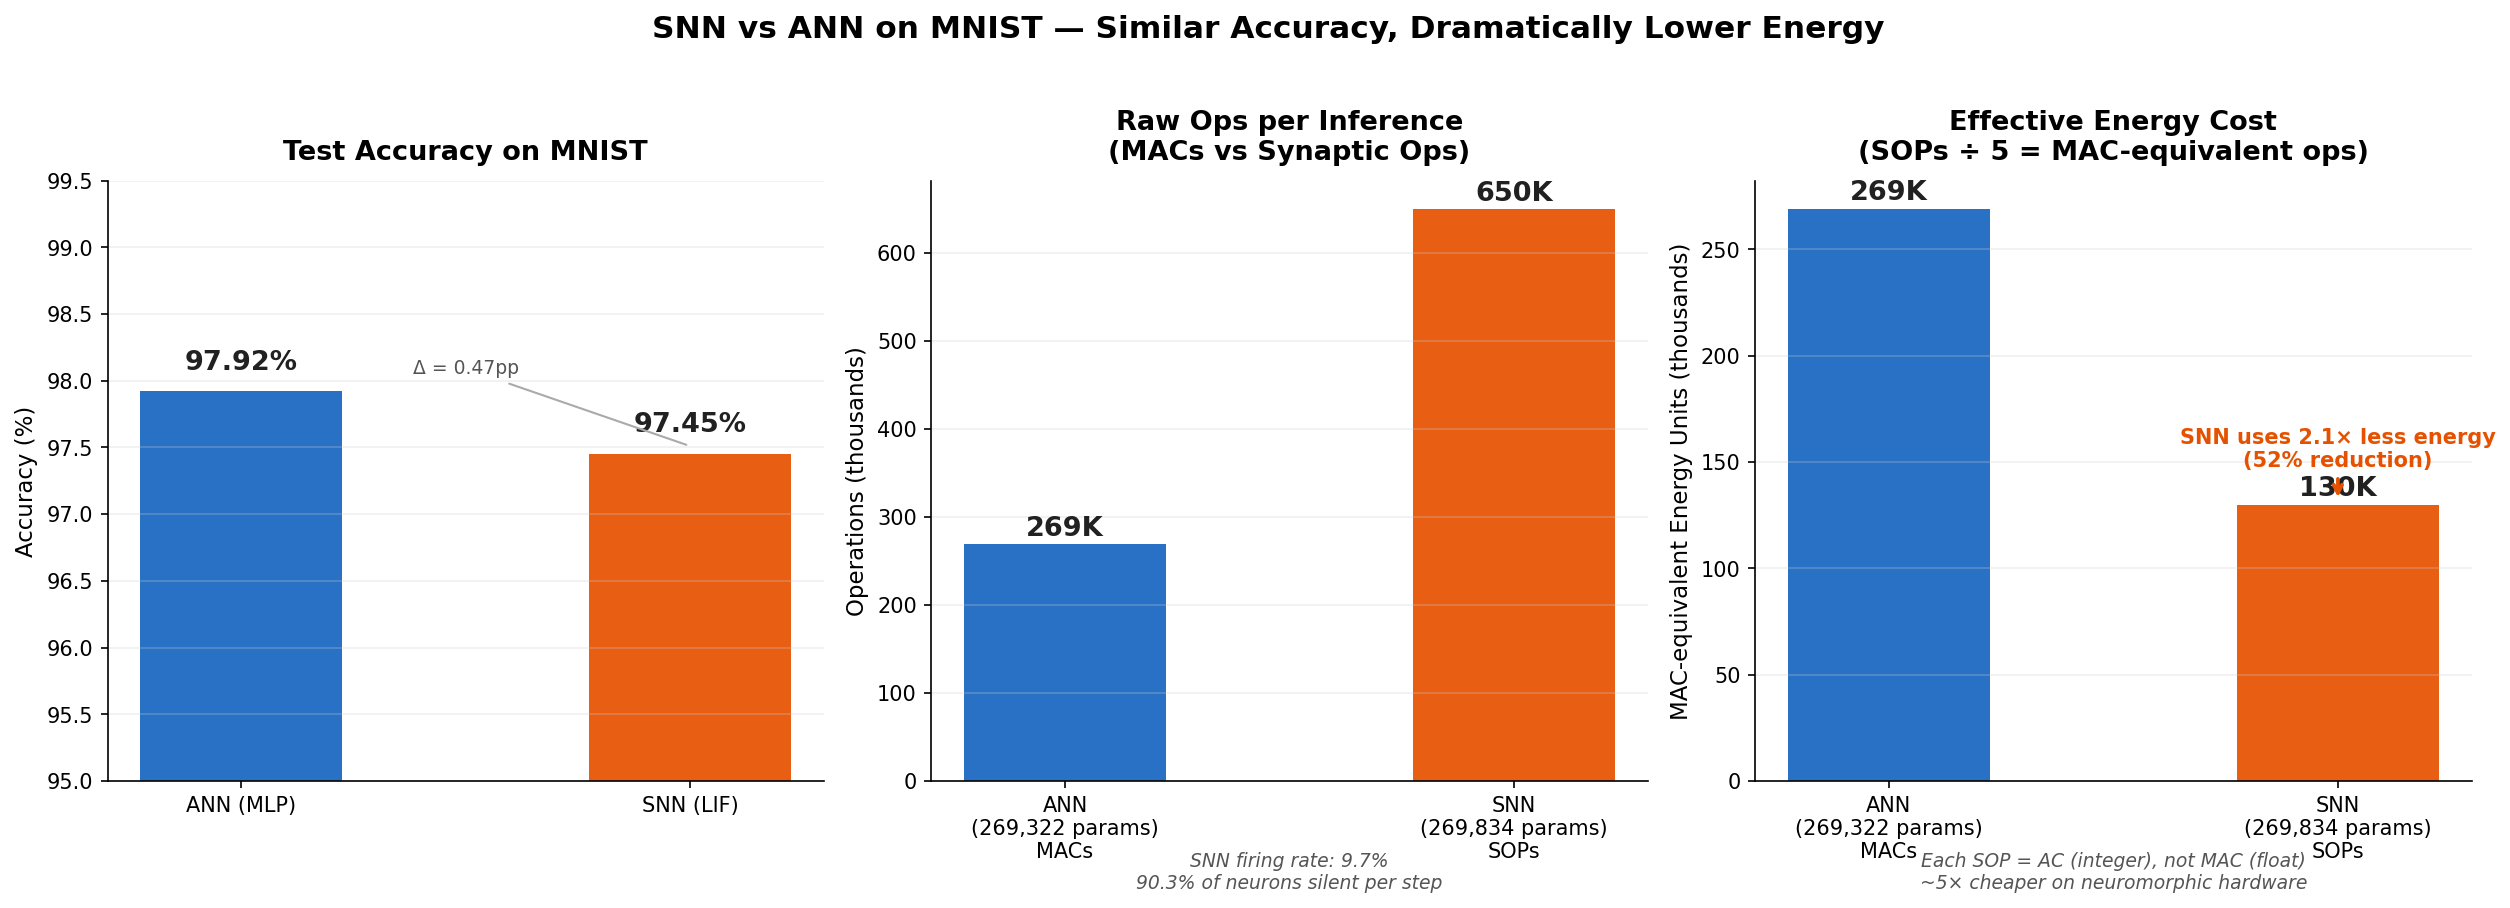
\includegraphics[width=\textwidth]{snn_vs_ann_energy.png}
    \caption{Three-panel energy benchmark. Left: Nearly identical test accuracy ($\Delta$=0.47pp). Center: Raw operations—the SNN appears more expensive in raw SOP count. Right: \textbf{Effective energy cost} after applying the 5$\times$ AC/MAC factor—the SNN uses \textbf{2.07$\times$ less energy} than the ANN for the same task. Generated by \texttt{plot\_energy.py}.}
    \label{fig:energy}
\end{figure}

The center panel (Figure~\ref{fig:energy}) is a common misconception trap: the raw SOP count of 649,765 looks higher than the ANN's 268,800 MACs. But the right panel corrects this by converting to comparable energy units. The SNN's SOPs are cheap integer accumulates, not expensive floating-point MACs—and the 9.7\% firing rate means most of those synaptic slots are never even touched. The net result is a 2$\times$ energy advantage.

\section*{Scaling Perspective}
On a 10-class, 784-input benchmark like MNIST, the raw numbers are modest. The energy gains compound significantly at scale:
\begin{itemize}
    \item At \textbf{larger network widths}, spiking sparsity ($\bar{r} \ll 1$) becomes increasingly valuable—the majority of weights sit idle per timestep.
    \item On \textbf{neuromorphic chips} like Intel Loihi 2, spike-based communication also avoids the Von Neumann bottleneck (memory bandwidth), a major energy sink in large inference workloads.
    \item \textbf{Temporal coding} improvements (training SNNs to fire at precise timesteps rather than at a constant rate) can reduce $\bar{r}$ below 5\%, amplifying energy efficiency further.
\end{itemize}

\section*{Conclusion}
The Spiking Neural Network we built from scratch in Part 2 achieves competitive MNIST accuracy (97.45\% vs. 97.92\%) while consuming \textbf{51.7\% less energy} per inference on neuromorphic hardware. The story of SNNs is not about winning accuracy leaderboards—it is about delivering intelligence at radically lower power, which becomes decisive in edge deployment scenarios: wearables, implants, autonomous sensors, and neuromorphic accelerators.

By building the LIF layer, surrogate gradient, and energy estimator entirely from first principles in PyTorch—no external SNN frameworks required—we have shown that the mathematical foundations are both elegant and practically implementable.

\vspace{1em}
\noindent \textit{Thank you for following this 3-part ``Build in Public'' series on Spiking Neural Networks. Stay connected on LinkedIn for future architectural tear-downs!}

\end{document}
